\scanpage{45}

\uline{Conjecture} 1) $H_B^i(X_C,C)$ est somme \inserted{directe} des sous-espaces engendrés par les \unsure{vecteurs} $\chi^{-p}$-propres, de façon intrinsèque ; posant, pour $p+q=i$
\[
H_B^{p,q}(X)_K=H_B^i(X_C,C)[p]^\pi
\]
on a une décomposition en \unsure{somme}
\[
\boxed{H_B^i(X_C,C)\simeq\coprod_{p+q=i}H_B^{p,q}(X)_K\otimes_K C[-p]}
\]

2) On a un isom canonique
\[
\boxed{\varphi_K^{pq}:H_B^{pq}(X)_K\simeq H^{p.q}(X)\overset{\mathrm{dfn}}{=}H^q(X,\Omega_X^p)}
\]

\figure{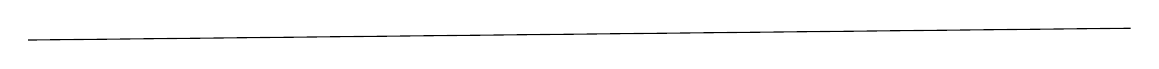
\begin{tikzpicture}\draw (0,0)--(14,0.15);\end{tikzpicture}}

\[
\begin{aligned}
\unsure{P_B|\rho_B}(z^i)&\in H_{\deleted{\unsure{B}}}^{2i}(X_C,\mathbb Z_p[i])^\pi
\subset H_B^{2i}(X_C,C)[i]^\pi=H_B^{i,i}(X)_K\\
&\phantom{\in H^{2i}(X_C,\mathbb Z_p[i])^\pi}\subset H_{\unsure{1}}^{2i}(X_C,\mathbb Z_p)
\end{aligned}
\]
\deleted{$\unsure{P_B|\rho_B}(z^i)$}
$\unsure{P_{DR}|\rho_{DR}}(z^i)\in H_{\deleted{\unsure{B}}}^{i,i}(X)$ ; on veut
\[
\boxed{\varphi_{\unsure{K}}^{ii}(\unsure{P_B|\rho_B}(z^i))=\unsure{P_{DR}|\rho_{DR}}(z^i)}
\]

\uline{NB.} On aura
\[
\unsure{P_B|\rho_B}(z^i)\in
\underbrace{H_B^{i,i}(\unsure{X_C,C})}_{\text{identifié à }H^{i,i}(X)}
\cap H^{2i}(X_C,\mathbb Z_p[i])
\]

\margin{55}
